%
% File acl2014.tex
%
% Contact: koller@ling.uni-potsdam.de, yusuke@nii.ac.jp
%%
%% Based on the style files for ACL-2013, which were, in turn,
%% Based on the style files for ACL-2012, which were, in turn,
%% based on the style files for ACL-2011, which were, in turn,
%% based on the style files for ACL-2010, which were, in turn,
%% based on the style files for ACL-IJCNLP-2009, which were, in turn,
%% based on the style files for EACL-2009 and IJCNLP-2008...

%% Based on the style files for EACL 2006 by
%%e.agirre@ehu.es or Sergi.Balari@uab.es
%% and that of ACL 08 by Joakim Nivre and Noah Smith

\documentclass[11pt]{article}
\usepackage[utf8]{inputenc}
\usepackage[french]{babel}
\usepackage{acl/acl2014}
\usepackage{times}
\usepackage{url}
\usepackage{latexsym}
\usepackage{graphicx}
\usepackage[colorlinks=true, allcolors=blue]{hyperref}

\graphicspath{{./fig/}{.}}

%\setlength\titlebox{5cm}

% You can expand the titlebox if you need extra space
% to show all the authors. Please do not make the titlebox
% smaller than 5cm (the original size); we will check this
% in the camera-ready version and ask you to change it back.


\title{Agents conversationnels à base de réseaux de neurones artificiels profonds}

\author{Guillaume Chevalier \\
  Université Laval \\ Baccalauréat en génie logiciel \\
  {\tt \small guillaume.chevalier.2@ulaval.ca} \\\And
  Samuel Cabral Cruz \\
  Université Laval \\ Baccalauréat en génie logiciel \\
  {\tt \small samuel.cabral-cruz.1@ulaval.ca}}

\date{}

\begin{document}
\maketitle

\begin{abstract}
Les approches par réseaux de neurones ont récemment surpassées les approches par algorithmes classiques pour ce qui en est des agents conversationnels, tels que Siri et Alexa, Google Assistant, Google Home
%[sources? Et est-ce que google assistant ca ce nomme comme ça? En fait j’ai aucune idée honnêtement si tous les agents que je vient de nommer fonctionnent avec des algos classiques ou pas.]
Plusieurs techniques sont apparues, ce qui cause……? Dans cet article, un survol des différentes techniques existantes est fait, de façon à ce que le lecteur ait une idée des différentes parties d’une architecture entièrement neurale pour les agents conversationnels.
\end{abstract}

\section{Introduction}
Au cours des années, différentes techniques sont apparues afin de créer des agents conversationnels. Classiquement, des approches algorithmiques étaient favorisées. Récemment, des approches par réseaux de neurones artificiels font leur apparition. Ainsi par exemple en 2014, un grand pas est fait lorsque les techniques par réseaux de neurones artificiels viennent à dépasser les performances des techniques classiques pour la tâche de faire de la traduction automatique \cite{attentionMechanism}. C’est de tels systèmes qui sont maintenant utilisés chez Google pour son outil Google Translate mis en production \cite{googleTranslate}. De plus, Google utilise des algorithmes de Speech-to-Text afin de pouvoir générer des sous-titres automatiquement pour les vidéos YouTube, et afin de pouvoir analyser les vidéos et les lier entre elles avec une approche sémantique
%TODO: TROUVER UN PAPER ICI: https://research.google.com/pubs/SpeechProcessing.html.
D’ailleurs, il est possible pour eux de générer de l’audio en temps réel avec une approche par réseaux de neurones convolutionnels \cite{wavenet}.


%EDIT: je parlerais d’IBM Watson, mais c’est une approche classique et c’est pas neuronal. C’est du 2014-2015, thought, donc ça se placerait bien dans l’intro. Faudrait trouver un de leurs papers ici, mais ça paraît que toute leur shit c’est des algos classiques, c’est décevant de leur part: http://researcher.watson.ibm.com/researcher/view_group_pubs.php?grp=2099



\section{Développement}
Toutes les parties nécessaires à concevoir une architecture de conversation neurale existent présentement. Un survol des meilleures architectures neuronales actuelles est fait.

\subsection{Traitement d'un intrant vocal}
La première étape de calcul au sein d’une architecture neurale destinée à comprendre et répondre à un utilisateur est de comprendre ce qu’il dit. Ainsi, il faut faire usage de techniques permettant la compréhension de ce que l’utilisateur dit, tel ce qui est fait avec les recherches par voix sur les engins de recherche les plus populaires, tels que notemment Google. Il est possible d’utiliser le réseaux de neurones TC-DNN-BLSTM-DNN, c’est-à-dire, des convolutions temporelles (TC) suivies de couches de neurones linéaires profondes (DNN), d’un LSTM Bidirectionnel (BLSTM) et puis d’un second DNN final \cite{acousticModeling}. Ainsi, cette architecture dépends d’un pré-traitement du signal par un autre algorithme lequel est plus classique et permet de transformer le signal en un domaine de fréquences personnalisé. C’est ce pré-traitement de l’information qui est introduit dans le réseau de neurones profond, afin d’en analyser le sens et de pouvoir convertir cela en états acoustiques, lesquels peuvent être convertis, cette fois, en texte littéraire. Cette architecture neurale est imagée à la Figure STT, et obtient un WER (Word Error Rate) de retranscription de 3.47, ce qui est présentement l’état de l’art (SOTA) sur le jeux de données et problème du Wall Street Journal (WSJ) eval’92 %[PAPER REQUIS POUR LE WSJ eval’92, CITATION].

%Figure STT: L’architecture neurale TC-DNN-BLSTM-DNN permet d’écouter le signal audio à l’aide des données audio extraites en fMMLR. Ainsi, un DNN suivi d’un BLSTM peut analyser ce signal pour classifier cela en états acoustiques, lesquels sont eux-mêmes repris par un algorithme classique qui permet de rassembler ces états en mots réels [DeepRecurrentNeuralNetworksForAcousticModelling]. Notons que cette architecture neural peut être utilisée pour raffiner le signal des mots prononcés, ce qui peut être envoyé directement dans un réseaux de neurones supérieur en tant que plongeage.

\subsection{Extraction des composantes de l'intrant et des sources d'information à analyser}
Une fois que la requête de l'utilisateur aura été convertie sous une forme textuelle facilement manipulable par un ordinateur, nous pourrions, dès lors, utiliser le plongement induit par l'étape précédente. Une autre approche consiste à reprendre cette sortie pour ensuite la fournir à une nouvelle structure qui se chargera d'aller extraire de nouvelles composantes qui aideront certainement à obtenir de meilleurs résultats pour la suite du processus. \\

À ce stade, nous devons comprendre que le signal est encore purement textuel et nous n'avons pour seule information qu'une décomposition des mots qui forment la demande reçue. Cependant, les langages sont formés de davantage de subtilités qu'un simple enchaînement de mots les uns après les autres. En effet, chaque mot joue un rôle précis dans la structure de la phrase et apporte une nuance particulière au contexte générale de celle-ci ou encore du texte avec une plus faible portée. C'est exactement ce que les travaux de ... visaient à faire. Ainsi, en ..., ce groupe de chercheurs a fait la publication d'un article détaillant leur approche fondée sur l'utilisation de réseaux de neurones. En plus de faire état de leurs travaux, ce groupe est aussi à l'origine d'outil qui est encore à ce jour considéré comme un incontournable: \cite{word2vec}. \\

Malgré le fait que cet article pour sur les approches neuronales, cet outil a plutôt fait la démonstration que des approches plus simplistes sont parfois plus adaptées. Comme le montre les figures \autoref{fig:skipgram} et \autoref{fig:cbow}, Word2vec se fonde sur la combinaison de deux approches nommées skip-gram et bag of words consistant simplement a. \\

\begin{figure}[ht]
  \centering
  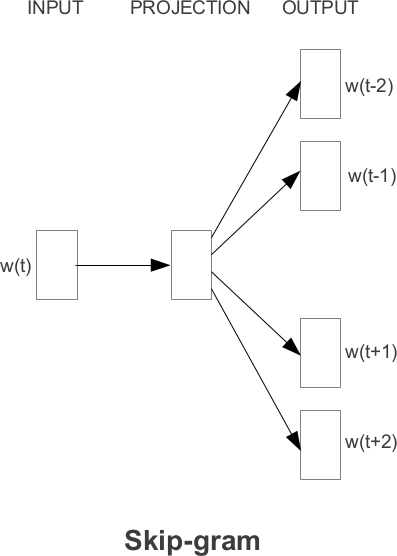
\includegraphics[width=\columnwidth]{skipgram}
  \caption{Architecture de la méthode de prédiction Skip-gram}
  \label{fig:skipgram}
\end{figure}

\begin{figure}[ht]
  \centering
  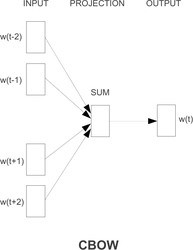
\includegraphics[width=\columnwidth]{cbow}
  \caption{Architecture de la méthode de prédiction CBOW}
  \label{fig:cbow}
\end{figure}

En fournissant la requête reçue à cet outil, il sera donc possible d'extraire les composantes sémantiques et syntaxiques sous-entendues par cette dernière. Par la suite, ces nouvelles composantes seront combinées à celle que nous avions déjà obtenues à l'étape précédente. En procédant avec cette seconde approche, nous réaliserons certainement un gain majeur au niveau de la performance des prochaines étapes en raison de l'ajout important de dimensionnalités qui fourniront beaucoup plus de flexibilité aux réseaux de neurones suivantes qui devront à leur tour détecter les nuances du langage. À titre d'exemple, lorsqu'un utilisateur demandera à l'assistant si ce dernier peut lui indiquer l'horaire du cinéma le plus prêt de sa position, l'assistant devra comprendre la nuance que ce qui intéresse vraiment l'utilisateur est l'horaire et non pas l'évaluation booléenne de sa capacité à s'acquitter de cette tâche. Par contre, dans le cas où l'utilisateur demanderait à l'assistant si ce dernier peut le connecté à l'Internet, l'assistant devra dans ce cas faire l'évaluation de sa capacité et répondre en par affirmation à notre cher utilisateur. \\
%TODO Référence au transfer learning

Mais qu'en est-il de nos sources d'informations? En fait, le processus entier bénéficiera certainement qu'un travail similaire soit fait à ce niveau aussi. Pour ce faire, deux approches s'offrent encore à nous. La première consistant encore une fois à utiliser word2vec et la seconde repose sur le même principe, mais à un niveau supérieur d'abstraction en considérant cette fois l'utilité de chacune des phrases dans le texte plutôt que de se concentrer sur le rôle de chaque mot dans chaque phrase.  \\

Il y a 2 façons d’avoir l’embedding du corpus de texte (ex: tout wikipédia) lequel sera utilisé pour répondre à la question. Word2vec et infersent. Expliquer les niveaux d’emedding de word2vec et infersent (word-level et sentence-level). Plugger ça dans un RNN ou autre chose, tel que vu à la section suivante.

\subsection{Interprêter la requête et cibler le contenu d'intérêt pour y répondre}
1. Mécanismes d’attention: expliquer et introduire les papers. Faire ca dans l’intro??
2. QA pur et dur

\subsection{Formulation d'une réponse à partir de l'information d'intérêt retenur}
Bien qu’il est intéressant de trouver l’endroit où porter attention dans un corpus textuel, il est tout autant intéressant de savoir comment générer une réponse textuelle à l’utilisateur. Cela peut être fait en utilisant le Hierarchical Recurrent Encoder-Decoder (HRED) tel qu’introduit par Iulian V. Serban et al. \cite{chatbot\string:HRED}. En effet, HRED est une imbrication hiérarchique de réseaux de neurones récurrents. Un premier est utilisé afin d’encoder les phrases, un second est utilisé afin de garder le contexte des réponses passées lesquelles ont déjà traitées, comme un suivi de la discussion dans une mémoire temporaire, et finalement un troisième RNN est utilisé afin de décoder l’information en une phrase en réponse à l’utilisateur. En insérant une telle architecture neurale dans les concepts précédemment introduits aux sections suivantes, il est possible de générer la réponse en retour à l’utilisateur en ayant le contexte de la question qu’il pose ainsi que le contexte des documents à parcourir avec les mécanismes d’attention, tel que décrit dans la section précédente sur la pose de question. Ainsi, le premier RNN du HRED qui encode l’information peut utiliser word2vec \cite{word2vec} directement, en plus d’utiliser un plongement (embedding) provenant de l’avant dernière couche de neurones du DNN (Deep Neural Network) de STT (Speech to Text). En plus de cela, il est possible d’utiliser le réseau de neurones infersent de Facebook \cite{inferSent}, lequel peut être concaténé au signal de sortie du RNN encodeur du HRED, en tant que plongement supplémentaire au niveau des phrases plutôt qu’au niveau des mots.

Dans une amélioration plus récente de l’architecture HRED \cite{chatbot\string:LVHRED}, il est possible d’utiliser une variable latente intermédiaire laquelle permet de faire le pont entre les réponses envoyées du décodeur vers l’utilisateur, en plus de réinjécter cette réponse dans l’encodeur qui écoute la réponse de l’utilisateur suite à cela. Cela permet non-seulement de garder encore plus de contexte d’une phrase à l’autre en passant le signal du décodeur à nouveau en feedback dans l’encodeur. Cela renforce la qualité de la requête attentionnelle laquelle peut être générée à la toute fin de l’encodeur du HRED. Ici pourrait alors s’insérer le mécanisme d’attention décrit dans la section précédente portant sur l’analyse de texte suite à des questions : une fois la question posée par l’utilisateur et lue dans l’encodeur, le HRED peut bénéficier de cette question dans son RNN intermédiaire, et cela en tant que requête attentionnelle à passer directement au système attentionnel, similairement à ce qui est fait dans les travaux de Karl Moritz Hermann et al. chez Google \cite{readNcomprehend}. Sommes toutes, le HRED aura accès à la question de l’utilisateur, et aura aussi accès au corpus de texte dans lequel il peut maintenant cibler l’information pertinente. Étant donné la taille énorme du corpus textuel dans lequel le réseaux de neurones peut lire l’information, tel que l’ensemble du texte sur Wikipédia par exemple, il est possible d’appliquer un MapReduce
%[premier paper ici: https://scholar.google.ca/scholar?hl=en&as_sdt=0%2C5&q=mapreduce&btnG= ]
pour analyser tout le texte très rapidement en un instant, et de façon distribuée sur plusieurs centaines d’ordinateurs lesquels utilisent eux-même les implémentations de word2vec et infersent définies plus haut sur le texte pour le lire, ainsi que la requête attentionnelle en tant que préalable. Cette partie, qui est distribuée et qui est surnommé le lecteur impatient, est représenté à la Figure TEACHING. Il y a même une amélioration possible sur cet architecture neurale. Il est visible dans la figure que plusieurs itérations entre la requête et le système attentionnel est fait. Cela devrait être fait en une seule étape afin de réduire la complexité algorithmique de linéaire à constante en fonction de la longueur de la requête, en termes de nombre de mots. La recherche suite à la requête pouvant être distribuée, cela peut être fait en un temps très rapide, tout comme les opérations décrites dans les sections précédentes.

%Figure TEACHING: Le lecteur impatient prends la requête “X visited England” afin de faire une recherche dans le texte “Mary went to England”, à l’aide du mécanisme d’attention lequel est ici dénoté “r”, assisté de la requête “u” [teachingMachinesReadComprehend].

\subsection{Retourner la réponse textuelle sous la forme d'un signal audio}
Une fois une réponse générée, il est intéressant de générer l’audio de cette à nouveau afin de répondre à l’utilisateur, ce qui est un autre calcul rapide qui peut se faire en temps réel. Cela est possible avec le CNN (Conv.. neural net) Wavenet d’Aaron van den Oord et al., développé chez Google \cite{wavenet}. En effet, il est possible de générer n’importe quel ton de voix avec Wavenet, ainsi le choix de la voix de la personne qui parle peut être fait par l’utilisateur. À titre d’exemple, cette architecture neurale est tellement puissante qu’il est possible de lui faire imiter la voix du président. Cette découverte récente par Google est la première fois qu’il est possible de confondre la voix pour une voix humaine réelle plutôt qu’une voix robotique, ainsi l’illusion est bien réussie. La façon dont Wavenet fonctionne est d’établir un préalable statistique (une variable conditionnée) qui est donnée à un premier algorithme qui s’occupe de trouver les bons tons de voix à générer avec Wavenet, à partir du texte. C’est ainsi que Wavenet, conditionné lui-même par le ton de voix demandé et par le texte, peut générer la voix de façon réalistique. C’est une méthode point par point, ainsi, chaque point dans la vague audio est généré en fonction des points précédents et du conditionnement demandé, c’est très bas niveau sur le signal qui est à un taux d’échantillonage de 16 kHz lors de l’entraînement, ce qui est assez pour capturer les subtilités de quelqu’un qui parlerait réellement dans un enregistrement. Cette phase générative est illustrée dans dans la Figure WAVENET.

%Figure WAVENET: À l’aide de convolutions causales dilatées, il est possible de prédire le prochain point dans la vague audio de façon efficace. Cela est un modèle autorégréssif : les points passés sont utilisés pour prédire les points suivants du même signal. Ainsi, la sortie est remise en entrée pour le calcul de l’étape suivante, ce sampling peut faire usage de mémoire cache, ce qui donne à cet algorithme générationnel un temps linéaire pour la génération, cela en fonction de la longueur du signal à générer [ref Paper Wavenet].

\section*{Conclusion}

\section*{Remerciements}

% include your own bib file like this:
\bibliographystyle{acl/acl}
\bibliography{bib/ref}


% \begin{figure*}
%   \centering
%   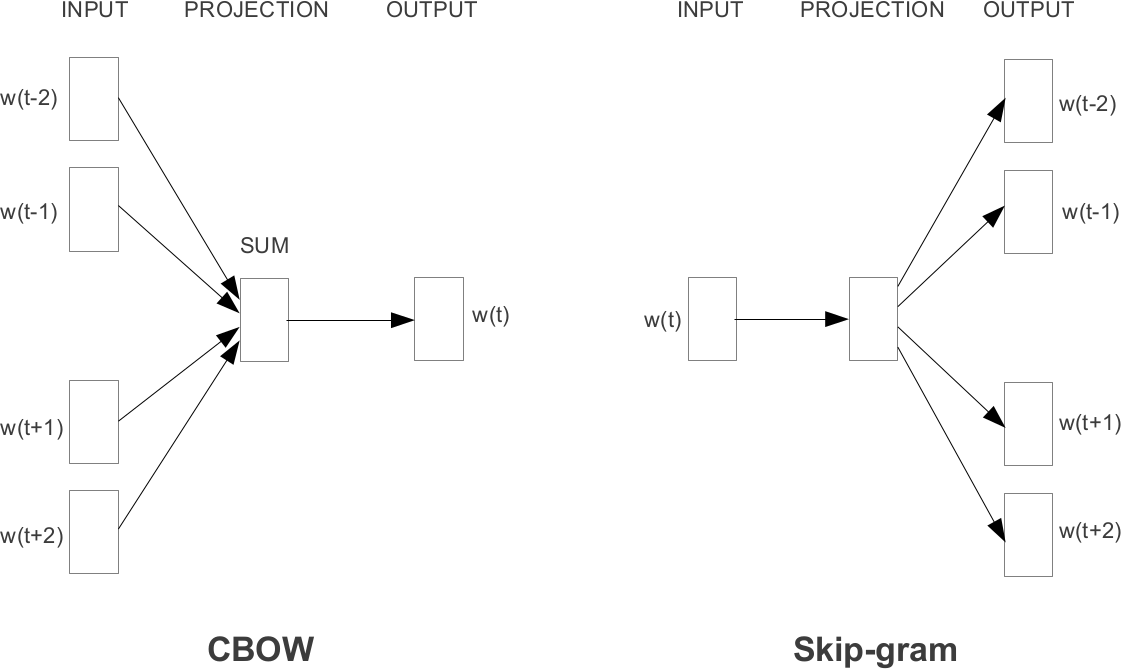
\includegraphics{word2vec}
% \end{figure*}

\end{document}
